\input{bmsLayoutPage}

\usetikzlibrary{angles, quotes, calc, babel}


\renewcommand{\bbwAufgabenBlockID}{AllgDreieck}

\renewcommand{\metaHeaderLine}{Allgemeines Dreieck}
\renewcommand{\arbeitsblattTitel}{Sinus- und Cosinussatz}

\ifisNURAUFGABEN
\renewcommand{\abplz}[1]{\vspace{1mm}}
\fi

\newcommand{\seitenUmbruchImAufgabenteil}{
\ifisNURAUFGABEN
\else
\noTRAINER{\newpage}
\fi
}%%

\begin{document}
\arbeitsblattHeader{}

\begin{center}V 0.2 (2026-02-12) \end{center}
\section{Teil 1: Aufgaben mit Skizzen}

Bei allen Aufgaben sind die Resultate auf drei signifikante Stellen zu runden.

\textit{Berechnen Sie die gesuchten Größen (markiert mit ?). Die Skizzen sind nicht maßstabsgetreu.}

\subsection*{A) Sinussatz: Seite berechnen}
\begin{minipage}[t]{0.48\textwidth}
    \begin{enumerate}[series=aufgaben]
        \item $b = ?$\\
        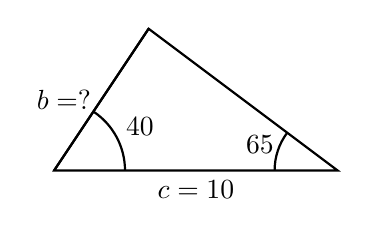
\begin{tikzpicture}[scale=1.2, thick]
            \coordinate (A) at (0,0); \coordinate (B) at (3,0); \coordinate (C) at (1,1.5);
            \draw (A) -- (B) node[midway, below]{$c=10$} -- (C) -- cycle;
            \draw (A) -- (C) node[midway, left]{$b=?$};
            \pic[draw, angle radius=0.9cm, "\,\,$40\degre$", angle eccentricity=1.3] {angle = B--A--C};
            \pic[draw, angle radius=0.8cm, "$65\degre$", angle eccentricity=1.3] {angle = C--B--A};
        \end{tikzpicture}
    \end{enumerate}
\end{minipage}
\hfill
\begin{minipage}[t]{0.48\textwidth}
    \begin{enumerate}[resume=aufgaben]
        \item $a = ?$\\
        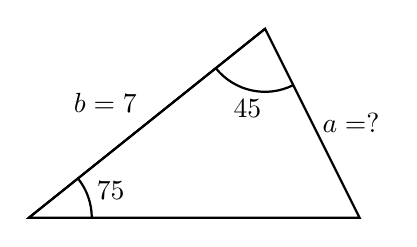
\begin{tikzpicture}[scale=1.2, thick]
            \coordinate (A) at (0,0); \coordinate (B) at (3.5,0); \coordinate (C) at (2.5,2);
            \draw (A) -- (B) -- (C) node[midway, right]{$a=?$} -- cycle;
            \draw (A) -- (C) node[midway, above left]{$b=7$};
            \pic[draw, angle radius=0.8cm, "\,\,$75\degre$", angle eccentricity=1.3] {angle = B--A--C};
            \pic[draw, angle radius=0.8cm, "$45\degre$", angle eccentricity=1.3] {angle = A--C--B};
        \end{tikzpicture}
    \end{enumerate}
\end{minipage}



\begin{enumerate}[resume=aufgaben]
    \item Gegeben sind in einem allgemeinen Dreieck $\gamma = 71\degre$, $b=5$ cm und $c=49$
    mm. Berechnen Sie Winkel $\alpha$ und Seite $a$.
    \item In einem allgemeinen Dreieck sind $\alpha=21\degre$, Seite
    $a=31$ mm und Seite $b=7.1$ cm. Berechnen Sie die fehlenden Seiten
    und Winkel.
\end{enumerate}



\TNTeop{}


\subsection*{B) Sinussatz: Winkel berechnen}
\begin{minipage}[t]{0.48\textwidth}
    \begin{enumerate}[resume=aufgaben]
        \item $\beta = ?$\\
        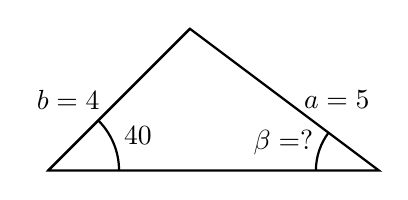
\begin{tikzpicture}[scale=1.2, thick]
            \coordinate (A) at (0,0); \coordinate (B) at (3.5,0); \coordinate (C) at (1.5,1.5);
            \draw (A) -- (B) -- (C) node[midway, right]{$\,\,a=5$} -- cycle;
            \draw (A) -- (C) node[midway, left]{$b=4\,\,$};
            \pic[draw, angle radius=0.9cm, "\,\,$40\degre$", angle eccentricity=1.3] {angle = B--A--C};
            \pic[draw, angle radius=0.8cm, "\hspace{-3mm}$\beta=?$", angle eccentricity=1.4] {angle = C--B--A};
        \end{tikzpicture}
    \end{enumerate}
\end{minipage}
\hfill
\begin{minipage}[t]{0.48\textwidth}
    \begin{enumerate}[resume=aufgaben]
        \item $\beta = ?$\\
        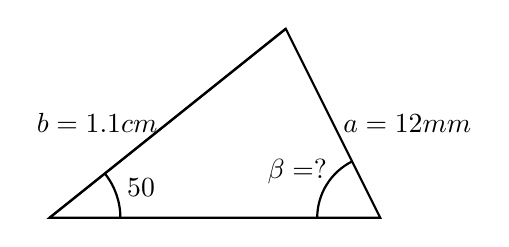
\begin{tikzpicture}[scale=1.2, thick]
            \coordinate (A) at (0,0); \coordinate (B) at (3.5,0); \coordinate (C) at (2.5,2);
            \draw (A) -- (B) -- (C) node[midway, right]{$a=12\text{ mm}$} -- cycle;
            \draw (A) -- (C) node[midway, left]{$b=1.1 \text{ cm}$};
            \pic[draw, angle radius=0.9cm, "\,\,$50\degre$", angle eccentricity=1.3] {angle = B--A--C};
            \pic[draw, angle radius=0.8cm, "$\hspace{-2mm}\beta=?$", angle eccentricity=1.4] {angle = C--B--A};
        \end{tikzpicture}
    \end{enumerate}
\end{minipage}

\TNTeop{}


\begin{minipage}[t]{0.48\textwidth}
    \begin{enumerate}[resume=aufgaben]
        \item $\alpha = ?$\\
        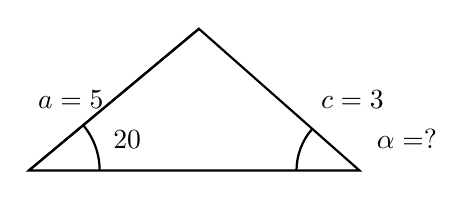
\begin{tikzpicture}[scale=1.2, thick]
            \coordinate (C) at (0,0); \coordinate (A) at (3.5,0); \coordinate (B) at (1.8,1.5);
            \draw (A) -- (B) -- (C) node[midway, right]{\hspace{25mm}$c=3$} -- cycle;
            \draw (B) -- (C) node[midway, left]{$a=5$};
            \pic[draw, angle radius=0.9cm, "\hspace{3mm}$20\degre$", angle eccentricity=1.3] {angle = A--C--B};
            \pic[draw, angle radius=0.8cm, "\hspace{33mm}$\alpha=?$", angle eccentricity=1.4] {angle = B--A--C};
        \end{tikzpicture}
    \end{enumerate}
\end{minipage}
\hfill
\begin{minipage}[t]{0.48\textwidth}
    \begin{enumerate}[resume=aufgaben]
        \item $\beta = ?$\\
        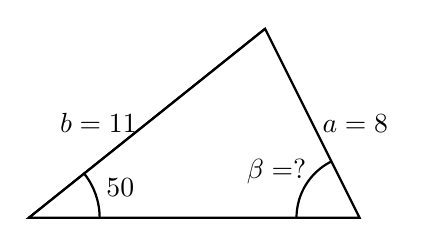
\begin{tikzpicture}[scale=1.2, thick]
            \coordinate (A) at (0,0); \coordinate (B) at (3.5,0); \coordinate (C) at (2.5,2);
            \draw (A) -- (B) -- (C) node[midway, right]{$a=8$} -- cycle;
            \draw (A) -- (C) node[midway, left]{$b=11$};
            \pic[draw, angle radius=0.9cm, "\,\,$50\degre$", angle eccentricity=1.3] {angle = B--A--C};
            \pic[draw, angle radius=0.8cm, "\hspace{-2mm}$\beta=?$", angle eccentricity=1.4] {angle = C--B--A};
        \end{tikzpicture}
    \end{enumerate}
\end{minipage}

\TNTeop{}





\subsection*{C) Sinussatz: Stumpfwinklige Dreiecke}
\begin{minipage}[t]{0.48\textwidth}
    \begin{enumerate}[resume=aufgaben]
        \item $\gamma = ?$ \\
        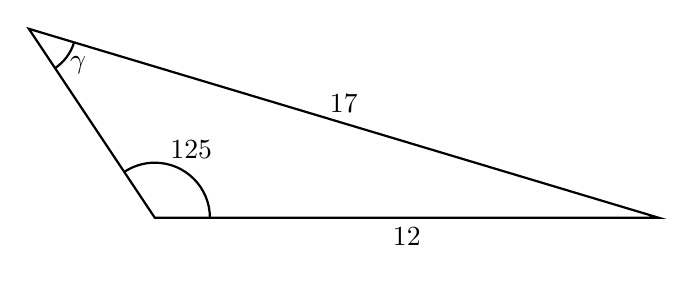
\begin{tikzpicture}[scale=1.6, thick]
            \coordinate (A) at (0,0); \coordinate (B) at (4,0); \coordinate (C) at (-1,1.5);
            \draw (A) -- (B) node[midway, below]{$12$} -- (C) node[midway, above]{$17$} -- cycle;
            \pic[draw, angle radius=0.7cm, "$125\degre$", angle eccentricity=1.4] {angle = B--A--C};
            \pic[draw, angle radius=0.6cm, "$\gamma$", angle eccentricity=1.3] {angle = A--C--B};
        \end{tikzpicture}
    \end{enumerate}
\end{minipage}
\hfill
\begin{minipage}[t]{0.48\textwidth}
    \begin{enumerate}[resume=aufgaben]
        \item $\alpha = ?$ \\
        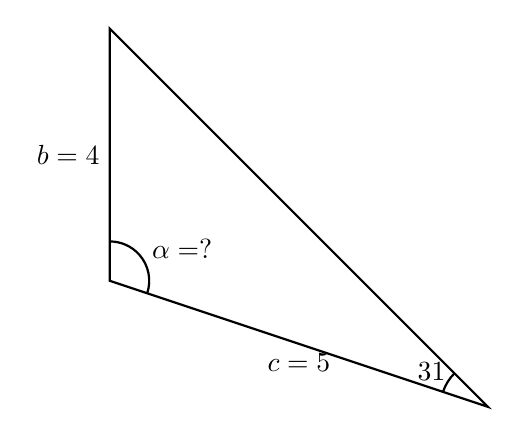
\begin{tikzpicture}[scale=1.6, thick]
            \coordinate (A) at (0,0); \coordinate (B) at (3,-1); \coordinate (C) at (0,2);
            \draw (A) -- (B) node[midway, below]{$c=5$} -- (C) -- cycle;
            \draw (C) -- (A) node[midway, left]{$b=4$} ;
            \pic[draw, angle radius=0.5cm, "\hspace{7mm}$\alpha=?$", angle eccentricity=1.4] {angle = B--A--C};
            \pic[draw, angle radius=0.6cm, "$31\degre$", angle eccentricity=1.4] {angle = C--B--A};
        \end{tikzpicture}
    \end{enumerate}
\end{minipage}

\vspace{0.5cm}

\begin{minipage}[t]{0.48\textwidth}
    \begin{enumerate}[resume=aufgaben]
        \item $\beta = ?$ \\
        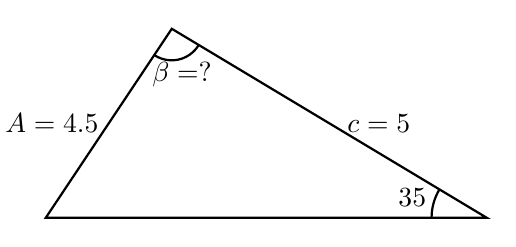
\begin{tikzpicture}[scale=1.6, thick]
            \coordinate (A) at (0,0); \coordinate (B) at (1,1.5); \coordinate (C) at (3.5,0);
            \draw (A) -- (B) node[midway, left]{\hspace{-4mm}$A=4.5$} -- (C) node[midway, right]{\hspace{1mm}$c=5$} -- cycle;
            \pic[draw, angle radius=0.4cm, "$\beta=?$", angle eccentricity=1.5] {angle = A--B--C};
            \pic[draw, angle radius=0.7cm, "$35\degre$", angle eccentricity=1.4] {angle = B--C--A};
        \end{tikzpicture}
    \end{enumerate}
\end{minipage}


\TNTeop{}



\subsection*{D) Cosinussatz: Seite berechnen}
\begin{minipage}[t]{0.48\textwidth}
    \begin{enumerate}[resume=aufgaben]
        \item $c = ?$\\
        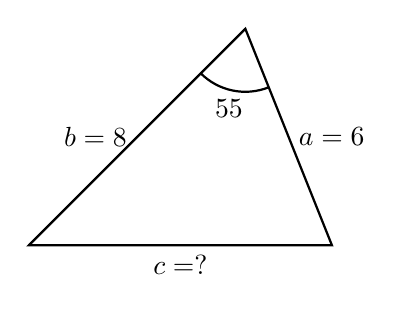
\begin{tikzpicture}[scale=1.1, thick]
            \coordinate (A) at (0,0); \coordinate (B) at (3.5,0); \coordinate (C) at (2.5,2.5);
            \draw (A) -- (B) node[midway, below]{$c=?$} -- (C) node[midway, right]{$a=6$} -- cycle;
            \draw (A) -- (C) node[midway, left]{$b=8$};
            \pic[draw, angle radius=0.8cm, "$55\degre$", angle eccentricity=1.3] {angle = A--C--B};
        \end{tikzpicture}
    \end{enumerate}
\end{minipage}
\hfill
\begin{minipage}[t]{0.48\textwidth}
    \begin{enumerate}[resume=aufgaben]
        \item $b = ?$\\
        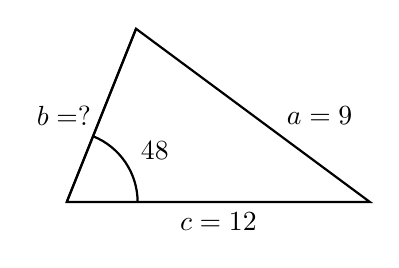
\begin{tikzpicture}[scale=1.1, thick]
            \coordinate (A) at (0,0); \coordinate (B) at (3.5,0); \coordinate (C) at (0.8,2);
            \draw (A) -- (B) node[midway, below]{$c=12$} -- (C) node[midway, right]{\hspace{3mm}$a=9$} -- cycle;
            \draw (A) -- (C) node[midway, left]{$b=?$};
            \pic[draw, angle radius=0.9cm, "\hspace{3mm}$48\degre$", angle eccentricity=1.3] {angle = B--A--C};
        \end{tikzpicture}
    \end{enumerate}
\end{minipage}

\TNTeop{}





\subsection*{E) Cosinussatz: Winkel berechnen}
\begin{minipage}[t]{0.48\textwidth}
    \begin{enumerate}[resume=aufgaben]
        \item $\alpha = ?$\\
        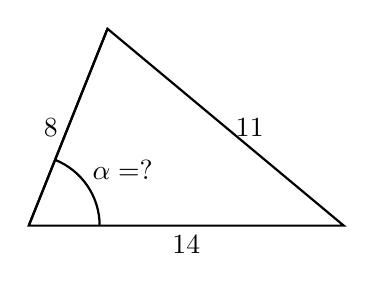
\begin{tikzpicture}[scale=1.0, thick]
            \coordinate (A) at (0,0); \coordinate (B) at (4,0); \coordinate (C) at (1,2.5);
            \draw (A) -- (B) node[midway, below]{$14$} -- (C) node[midway, right]{$11$} -- cycle;
            \draw (A) -- (C) node[midway, left]{$8$};
            \pic[draw, angle radius=0.9cm, "\hspace{3mm}$\alpha=?$", angle eccentricity=1.4] {angle = B--A--C};
        \end{tikzpicture}
    \end{enumerate}
\end{minipage}
\hfill
\begin{minipage}[t]{0.48\textwidth}
    \begin{enumerate}[resume=aufgaben]
        \item $\gamma = ?$\\
        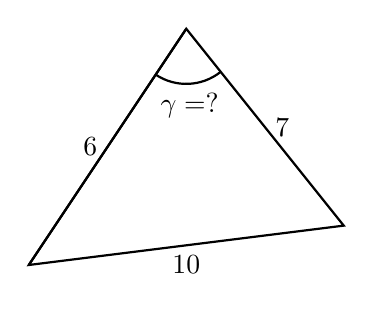
\begin{tikzpicture}[scale=1.0, thick]
            \coordinate (A) at (0,0); \coordinate (B) at (4,0.5); \coordinate (C) at (2,3);
            \draw (A) -- (B) node[midway, below]{$10$} -- (C) node[midway, right]{$7$} -- cycle;
            \draw (A) -- (C) node[midway, left]{$6$};
            \pic[draw, angle radius=0.7cm, "$\gamma=?$", angle eccentricity=1.4] {angle = A--C--B};
        \end{tikzpicture}
    \end{enumerate}
\end{minipage}

\TNTeop{}



\subsection*{F) Vermischte Aufgaben mit Skizzen}
\begin{minipage}[t]{0.32\textwidth}
    \begin{enumerate}[resume=aufgaben]
        \item $x = ?$ \\
        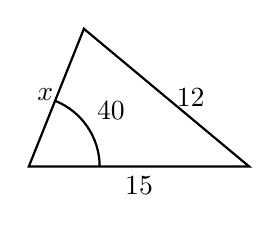
\begin{tikzpicture}[scale=0.7, thick]
            \coordinate (A) at (0,0); \coordinate (B) at (4,0); \coordinate (C) at (1,2.5);
            \draw (A) -- (B) node[midway, below]{$15$} -- (C) node[midway, right]{$12$} -- cycle;
            \pic[draw, angle radius=0.9cm, "$40\degre$", angle eccentricity=1.4] {angle = B--A--C};
            \node at (0.3, 1.3) {$x$};
        \end{tikzpicture}
    \end{enumerate}
\end{minipage}
\hfill
\begin{minipage}[t]{0.32\textwidth}
    \begin{enumerate}[resume=aufgaben]
        \item $\beta = ?$ \\
        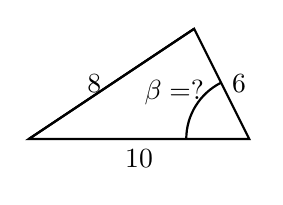
\begin{tikzpicture}[scale=0.7, thick]
            \coordinate (A) at (0,0); \coordinate (B) at (4,0); \coordinate (C) at (3,2);
            \draw (A) -- (B) node[midway, below]{$10$} -- (C) node[midway, right]{$6$} -- cycle;
            \draw (A) -- (C) node[midway, left]{$8$};
            \pic[draw, angle radius=0.8cm, "$\beta=?$", angle eccentricity=1.4] {angle = C--B--A};
        \end{tikzpicture}
    \end{enumerate}
\end{minipage}
\hfill
\begin{minipage}[t]{0.32\textwidth}
    \begin{enumerate}[resume=aufgaben]
        \item $y = ?$ \\
        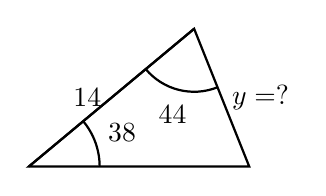
\begin{tikzpicture}[scale=0.7, thick]
            \coordinate (A) at (0,0); \coordinate (B) at (4,0); \coordinate (C) at (3,2.5);
            \draw (A) -- (B) -- (C) node[midway, right]{$y=?$} -- cycle;
            \draw (A) -- (C) node[midway, left]{$14$};
            \pic[draw, angle radius=0.9cm, "$38\degre$", angle eccentricity=1.4] {angle = B--A--C};
            \pic[draw, angle radius=0.8cm, "$44\degre$", angle eccentricity=1.4] {angle = A--C--B};
        \end{tikzpicture}
    \end{enumerate}
\end{minipage}

\vspace{0.8cm}

\begin{minipage}[t]{0.32\textwidth}
    \begin{enumerate}[resume=aufgaben]
        \item $\alpha = ?$ \\
        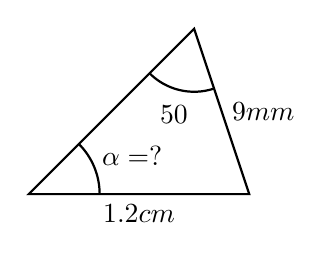
\begin{tikzpicture}[scale=0.7, thick]
            \coordinate (A) at (0,0); \coordinate (B) at (4,0); \coordinate (C) at (3,3);
            \draw (A) -- (B) node[midway, below]{$1.2 \text{ cm}$} --
        (C) node[midway, right]{$9 \text{ mm}$} -- cycle;
            \pic[draw, angle radius=0.9cm, "\hspace{3mm}$\alpha=?$", angle eccentricity=1.4] {angle = B--A--C};
            \pic[draw, angle radius=0.8cm, "$50\degre$", angle eccentricity=1.4] {angle = A--C--B};
        \end{tikzpicture}
    \end{enumerate}
\end{minipage}
\hfill
\begin{minipage}[t]{0.32\textwidth}
    \begin{enumerate}[resume=aufgaben]
        \item $z = ?$ \\
        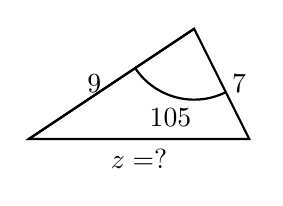
\begin{tikzpicture}[scale=0.7, thick]
            \coordinate (A) at (0,0); \coordinate (B) at (4,0); \coordinate (C) at (3,2);
            \draw (A) -- (B) node[midway, below]{$z=?$} -- (C) node[midway, right]{$7$} -- cycle;
            \draw (A) -- (C) node[midway, left]{$9$};
            \pic[draw, angle radius=0.9cm, "$105\degre$", angle eccentricity=1.3] {angle = A--C--B};
        \end{tikzpicture}
    \end{enumerate}
\end{minipage}
\hfill
\begin{minipage}[t]{0.32\textwidth}
    \begin{enumerate}[resume=aufgaben]
        \item $\epsilon = ?$ \\
        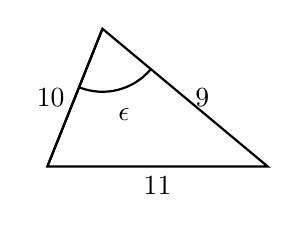
\begin{tikzpicture}[scale=0.7, thick]
            \coordinate (A) at (0,0); \coordinate (B) at (4,0); \coordinate (C) at (1,2.5);
            \draw (A) -- (B) node[midway, below]{$11$} -- (C) node[midway, right]{$9$} -- cycle;
            \draw (A) -- (C) node[midway, left]{$10$};
            \pic[draw, angle radius=0.8cm, "$\epsilon$", angle eccentricity=1.4] {angle = A--C--B};
        \end{tikzpicture}
    \end{enumerate}
\end{minipage}

\vspace{1cm}

\TNTeop{}



\section*{Teil 2: Vermischte Aufgaben in Textform}
\textit{Skizzieren Sie das Dreieck $ABC$ zuerst selbstständig.}

\begin{enumerate}[resume=aufgaben]
    \item Gegeben sind $a = 5.4$ cm, $b = 7.2$ cm und $c = 9.0$ cm. Berechnen Sie den Winkel $\beta$.
    \item Im Dreieck $ABC$ sind $b = 12$ m, $\beta = 45\degre$ und $\gamma = 70\degre$. Berechnen Sie die Länge der Seite $c$.
    \item Gegeben sind $a = 8.5$ cm, $c = 6.2$ cm und der eingeschlossene Winkel $\beta = 115\degre$. Berechnen Sie die Seite $b$.
    \item Im Dreieck sind $b = 15$ cm, $c = 10$ cm und $\gamma = 30\degre$ gegeben. Berechnen Sie $\beta$.
    \item Gegeben sind $a = 12$ cm, $b = 16$ cm und $\alpha = 35\degre$. Berechnen Sie $c$.
    \item In einem Dreieck sind $a=6, b=7$ und $\alpha=40\degre$. Berechnen Sie den Winkel $\gamma$.
\end{enumerate}

\TNTeop{}

\newpage

\textit{Skizzieren Sie vorab.}

\begin{enumerate}[resume=aufgaben]
    \item Ein Grundstück hat die Form eines Vierecks ABCD.\\
    Berechnen Sie aus den folgenden Angaben den Flächeninhalt dieses
    Grundstückes:

Winkel $BDC = 32.1\degre$, Winkel $ADB = 89.3\degre$, Seite $CD=14$ m,
Winkel $DCA=48.3\degre$, Winkel $ACB = 92.5\degre$

\end{enumerate}

\TNTeop{}
%%%%%%%%%%%%%%%%%%%%%%%%%%%%%%%%%%%%%%%%%%%%%%%%%%%%%%%%%%%%%%%%%%%%%5
\section*{Lösungen}
\begin{minipage}[t]{0.45\textwidth}
\begin{enumerate}[series=loesungen]
    \item $b \approx 9.38$
    \item $a \approx 7.81$
    \item \textbf{Zweideutig} $\alpha_1 \approx  34.2\degre $,
    $\alpha_2 \approx 3.76\degre $, $a_1 \approx 29.2$ mm, $a_2 \approx 3.39$ mm
    \item \textbf{Zweideutig} $\beta_1 \approx  55.2\degre $,
    $\beta_2 \approx 125.\degre $,$\gamma_1 \approx  104.\degre $,
    $\gamma_2 \approx 34.2\degre $, $c_1 \approx 84.0$ mm, $c_2 \approx 48.6$ mm
    \item $\beta \approx 31.0\degre$
    \item $\beta \approx 44.6\degre$
    \item  \textbf{Zweideutig} $\alpha \approx 34.8\degre$ od. $\approx 145.\degre$
    \item \textit{keine Lösung: ($\sin \beta > 1$)}
    \item $\gamma \approx 35.3\degre$
    \item \textbf{Zweideutig}  $\alpha \approx 109.\degre$ od. $9.08\degre$
    \item \textbf{Zweideutig}  $\beta \approx 105.\degre$ od. $4.59\degre$
    \item $c \approx 6.70$
    \item \textbf{Zweideutig}  $b \approx 9.24$ od. $6.82$
    \item $\alpha \approx 51.6\degre$
\end{enumerate}
\end{minipage}
\hfill
\begin{minipage}[t]{0.45\textwidth}
\begin{enumerate}[resume=loesungen]
    \item $\gamma \approx 100.\degre$
    \item \textbf{Zweideutig}  $x \approx 4.35$ od. $18.6$
    \item $\beta \approx 53.1\degre$
    \item $y \approx 8.70$
    \item $\alpha \approx 35.1\degre$
    \item $z \approx 12.8$
    \item $\epsilon \approx 70.5\degre$
    \item $\beta \approx 53.1\degre$
    \item $c \approx 16.0$ m
    \item $b \approx 12.5$ cm
    \item \textbf{Zweideutig:}  $\beta \approx 48.6\degre$ od. $131.\degre$
    \item \textbf{Zweideutig:} $c \approx 20.8$ od. $5.38$
    \item \textbf{Zweideutig:} $\gamma \approx 91.4\degre$
    od. $8.6\degre$
    \item Fläche $\approx 2.36 \cdot{} 10^3 \text{ m}^2$
\end{enumerate}
\end{minipage}


\end{document}%
